\chapter{Ballerina}	%The main chapter title
\chaptermark{Ballerina}	%Short version for page header. Comment if not needed
\label{Chapter3}

Neste capitulo será explorado a linguagem de programação \textit{Ballerina}. Será feita uma introdução a mesma, enumerando as características distintivas, bem como é estruturado um projeto, como é construir, testado e implementado um serviço \textit{web}.

\section{Apresentação}

\textit{Ballerina}, é uma linguagem \textit{open source}, projetada pela empresa \ac{wso2} e que teve o seu lançamento no ano de 2019, visa facilitar o desenvolvimento de aplicações modernas baseadas em nuvem, ou seja, serviços altamente escaláveis e orientados a conexão. Apresenta várias semelhanças, com as linguagens C, C++, Java e JavaScript.

\textit{Ballerina} não é só uma linguagem de programação, mas sim um ecossistema, esta disponibiliza também um repositório no qual, este contém vários pacotes oficiais como pacotes feitos pela comunidade, que podem ser utilizados pelos desenvolvedores para facilitar a implementação de um certo problema, como, por exemplo, \textit{drivers} de bases de dados, autenticação, criptografia, entre outros. Também é uma maneira dos desenvolvedores poderem, gerir versões, verificar alterações nos pacotes e resolver conflitos de dependências entre pacotes. A esse repositório é-lhe dado o nome de \textit{Ballerina Central} \cite{centralBallerina}.

\section{Características}

Sendo que, \textit{Ballerina} recorre a um modelo de recorrência baseado em mensagens, cada serviço é executado simultaneamente, dado que, cada um deles é executado num processo.

Outra das suas caraterísticas é que esta é estaticamente tipada, o que significa que o tipo de uma variável é determinado em tempo de compilação e permanece o mesmo durante a execução do programa. Isso permite a capacidade de identificar problemas durante a compilação, o que pode reduzir o tempo e evitar que ocorram problemas durante a execução do programa. Por exemplo, se uma variável tiver sido definida como um inteiro e tentarmos atribuir-lhe uma \textit{string}, o compilador indicará um erro durante a compilação e não durante a execução \cite{tiposBallerina}.

Em \textit{Ballerina}, os dados são tratados como os outros tipos de dados funcionais como \textit{strings} e inteiros, dado que, são-lhes concedidos a mesma importância, permitindo que os desenvolvedores os manipulem e criem sem grande esforço. Uma das formas de isso ser obtido é mediante tipos de dados compostos como registos e objetos, aliados aos recursos de manipulação dos mesmos, como mapeamentos e filtros, que ajudam a processar um conjunto de informações grandes de forma eficiente e eficaz.

Comparando com outras linguagens, tem uma particularidade, no qual, é possível por meio de fluxogramas visualizar e a compreender o fluxo de dados num programa. Por outro lado, também pode servir para se entender como é feita a comunicação entre serviços.

E por último, tem suporte nativo com os formatos \textit{JSON} e \textit{XML}. \cite{ballerina}

\section{Estrutura de um projeto}
Um projeto em \textit{Ballerina} é organizado numa única unidade compartilhável denominada pacote. Por sua vez, um pacote pode ser constituído por vários módulos. Cada módulo é um conjunto de ficheiros do código-fonte, testes e recursos. É comum um projeto pequeno só ter um, mas à medida que o projeto vai ficando mais complexo nasce a necessidade de se criar mais, para melhor organizar o código e separar responsabilidades. Vale a pensa mencionar que cada ficheiro desta linguagem é acompanhado por uma extensão \textit{.bal} \cite{organizacaoCodigo}. Na figura \ref{fig:estruturaProjeto} é demonstrado um exemplo simples daquilo que foi mencionado em cima. 

\begin{figure}[H]
	\centering
	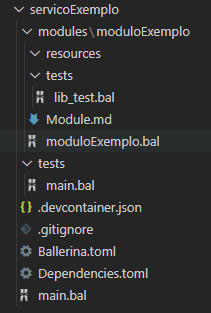
\includegraphics[scale=0.8]{estruturaProjeto}
	\caption{Exemplo da estrutura de um projeto.}
	\label{fig:estruturaProjeto}
\end{figure}

\section{Suporte num \ac{ide}}

O ambiente de desenvolvimento aconselhado para o desenvolvimento de código \textit{Ballerina} é o \ac{vsc}, dado, a sua integração nativa com a linguagem. Adicionalmente, esta disponibiliza uma extensão que auxilia o programador no desenvolvimento de código, uma vez que, disponibiliza funcionalidades tais como, correção de erros, \textit{noteboooks}, preenchimento automático de código e representação gráfica do código \cite{addon}.

\section{Implementar serviços na \textit{cloud}}
Feito o código necessário, este precisa de passar por um processo de implementação para passar a produção e começar a ser usado pelo utilizador final do sistema. Esse programa pode ser implementado na \textit{cloud} por meio de contentores \textit{docker} ou \textit{kubernetes}, para gerir e escalar os serviços em nuvens públicas ou privadas. Este processo descrito anteriormente, pode ser automatizado e simplificado com os recurso disponibilizados da linguagem, facilitando desta forma, o processo de implementação num ambiente de produção e fazendo com que, os desenvolvedores se concentrem mais a desenvolver os serviços do que com a implementação desses mesmos \cite{codeCloud}.

\section{Exemplos}
\subsection{Criação de um serviço}

Na Listagem \ref{lst:examplo1}, o código descrito importa o módulo \textit{HTTP}, que contém as funções para encarregar-se com pedidos \textit{HTTP}. Posteriormente, é criado um serviço que ouve pedidos na porta 9090 e na qual contém uma função do tipo \textit{GET} com o nome \textit{greeting} e que retorna uma \textit{string} \textit{"Hello, World"}.

\begin{minipage}{0.9\linewidth}
\begin{lstlisting}[language=ballerina, caption=Exemplo de um serviço. \cite{exemploB1}, label=lst:examplo1]
import ballerina/http;

service on new http:Listener(9090) {
    resource function get greeting() returns string {
        return "Hello, World!";
    }
}
\end{lstlisting}
\end{minipage}

\subsection{Conexão à base de dados}

Na Listagem \ref{lst:examplo4}, o código descrito importa o módulo \textit{MySQL} que contém funções que permitem o acesso a uma base de dados. Posteriormente é inicializado um cliente MySQL com as configurações necessárias, o anfitrião, o nome de utilizador, a palavra-passe e a porta. É importante mencionar que estes dados deveriam estar num ficheiro à parte e no qual seriam chamados. Para realizar isso seria preciso criar um ficheiro com o nome \textit{Config.toml} \cite{v}. 

Já na função \textit{init()}, nesta é instanciado um novo cliente MySQL, cujo objetivo é criar uma base de dados através da função \textit{execute()} com a respetiva \textit{query}. Ao criar-se a base de dados, já é possível criar-se uma tabela, visto isso, é utilizada outra instância já declarada anteriormente para interagir com a base de dados e executar comandos SQL na mesma. A tabela criada tem duas colunas, \textit{ingredient\_id} (declarado como inteiro, é a chave primária e incrementa automaticamente) e \textit{designation} (declarado como string).

\begin{minipage}{0.9\linewidth}
\begin{lstlisting}[language=ballerina, caption=Exemplo de uma coneção a base de dados. , label=lst:examplo4]
import ballerinax/mysql;
import ballerinax/mysql.driver as _; 
import ballerina/sql;

string USER = "myUser";
string PASSWORD = "myPassword";
string HOST = "localhost";
int PORT = 3306;

final mysql:Client dbClient;

function init() returns error? {
    mysql:Client dbClientCreate = check new(host=HOST, user=USER, password=PASSWORD, port=PORT);
    sql:ExecutionResult _ = check dbClientCreate->execute(`CREATE DATABASE IF NOT EXISTS Ingredient`);
    check dbClientCreate.close();
    dbClient = check new(host=HOST, user=USER, password=PASSWORD, port=PORT, database="Ingredient"); 
    sql:ExecutionResult _ = check dbClient->execute(`CREATE TABLE IF NOT EXISTS Ingredient.Ingredients (
                    ingredient_id INT AUTO_INCREMENT,
                    designation VARCHAR(255), 
                    PRIMARY KEY (ingredient_id)
                                         )`);                                
}
\end{lstlisting}
\end{minipage}

\subsection{Uso do \textit{RabbitMQ}}

Na Listagem \ref{lst:examplo5}, o código descrito importa o módulo \textit{RabbitMQ} que contém funções que permitem realizar a comunicação entre serviços.

Na função \textit{main()} é instanciado um novo cliente \textit{RabbitMQ}, no qual, são definidas o \textit{host} e porta de acesso ao servidor. E finalmente através da função \textit{queueDeclare} é criada uma \textit{queue} com o nome \textit{"TestQueue"}.

\begin{minipage}{0.9\linewidth}
\begin{lstlisting}[language=ballerina, caption=Exemplo de criação de uma queue. , label=lst:examplo5]
import ballerinax/rabbitmq;

public function main() returns error? {
    rabbitmq:Client client = check new (rabbitmq:DEFAULT_HOST, rabbitmq:DEFAULT_PORT);
    check client->queueDeclare("TestQueue");
}
\end{lstlisting}
\end{minipage}

Na Listagem \ref{lst:examplo6}, como na listagem anterior, importa o módulo \textit{RabbitMQ} e o módulo \textit{HTTP}. O presente código é um exemplo de como combinar um serviço \textit{web} com \textit{RabbitMQ}. Começa-se por declarar um registo \textit{"Test"}, que descreve um objeto, será este o objeto enviado na mensagem para o servidor. Depois disso é feita a declaração do serviço juntamente da porta em que ouvirá os pedidos. Dentro deste são instanciados um cliente \textit{RabbitMQ} e descritas duas funções. A  função \textit{"init"} é usada para inicializar uma conexão com o servidor, e a função \textit{"tests"} é responsável por receber o pedido do cliente \textit{web} e publicá-lo na \textit{queue} \textit{"TestQueue"} criada anteriormente na listagem \ref{lst:examplo5}.

\begin{minipage}{0.9\linewidth}
\begin{lstlisting}[language=ballerina, caption=Exemplo de publicação de mensagem para o servidor. , label=lst:examplo6]
import ballerina/http;
import ballerinax/rabbitmq;

type Test readonly & record {
    int id;
    string name;
};

service / on new http:Listener(9092) {
    private final rabbitmq:Client client;
    function init() returns error? {
        self.client = check new (rabbitmq:DEFAULT_HOST, rabbitmq:DEFAULT_PORT);
    }
    resource function post tests(Test test) returns http:Accepted|error {
        check self.client->publishMessage({
            content: test,
            routingKey: "TestQueue"
        });

        return http:ACCEPTED;
    }
}
\end{lstlisting}
\end{minipage}

Na Listagem \ref{lst:examplo7}, como na listagem anterior, importa o módulo \textit{RabbitMQ} e o módulo \textit{Log}. Começa-se por declarar um registo \textit{"Test"}, que descreve um objeto, será este o objeto recebido na mensagem enviada pelo servidor. 

Na função \textit{main()} é declarado um novo cliente \textit{RabbitMQ} com o \textit{host} e porta de acesso ao servidor. A seguir, a mensagem enviada é consumida através da função \textit{consumePayload()} da \textit{queue} \textit{"TestQueue"}. Depois do objeto \textit{"Test"} ser validado, uma mensagem aparecerá na consola devido à função \textit{"printInfo"} disponibilizada pelo módulo \textit{Log}.

\begin{minipage}{0.9\linewidth}
\begin{lstlisting}[language=ballerina, caption=Exemplo da consumição de uma mensagem do servidor. , label=lst:examplo7]
import ballerina/log;
import ballerinax/rabbitmq;

public type Test record {
    int id;
    string name;
};

public function main() returns error? {
    rabbitmq:Client client = check new (rabbitmq:DEFAULT_HOST, rabbitmq:DEFAULT_PORT);
    Test 'test = check client->consumePayload("TestQueue");
    if 'test.isValid {
        log:printInfo(string `Received valid test for ${'test.name}`);
    }
}
\end{lstlisting}
\end{minipage}

\subsection{Concorrência}

Na Listagem \ref{lst:examplo2}, o código descrito importa o módulo \textit{io}, que contém módulos de interação com ficheiros e módulos de \textit{output} e \textit{input}. É definido um registo com o nome \textit{"Person"} com dois campos, \textit{"name"} e \textit{"employed"} sendo os seus tipos, \textit{string} e \textit{boolean}, respetivamente. Também define uma função chamada \textit{"process"} que recebe dois parâmetros, uma lista de objetos \textit{"Person"} com o nome \textit{"members"} e uma lista de inteiros com o nome \textit{"quantities"}.

Na função descrita referida anteriormente, esta utiliza dois \textit{workers} para processar os dados recebidos como parâmetros na função. No caso do \textit{worker} com denominação "w1" é feito uma contagem dos membros empregado através do parâmetro \textit{"employed"} de cada objeto \textit{"Person"} na lista \textit{"members"}, essa contagem é envida a seguir para o \textit{worker} com denominação "w2" através do uso da ação (->) e conclui enviando um mensagem do tipo \textit{string} para o \textit{endpoint} da função com o valor contabilizado. Por outro lado, no w2, é inicialmente feito a soma de todos os valores recebidos no parâmetro \textit{"quantities"} e fica a espera do resultado retornado pelo "w1", recorrendo a ação (<-), dado esse recebimento, é a seguir calculado a média para os membros empregados e conclui enviando um mensagem do tipo \textit{string} para o \textit{endpoint} da função com esse valor calculado.

Após a definição do "w1" e "w2", a função fica à espera dos valores de cada \textit{worker} e imprime-as usando a função \textit{io:println}.

\begin{minipage}{0.9\linewidth}
\begin{lstlisting}[language=ballerina, caption=Exemplo de concorrência. \cite{exemploB2}, label=lst:examplo2]
import ballerina/io;

type Person record {|
    string name;
    boolean employed;
|};

function process(Person[] members, int[] quantities) {
    worker w1 {
        Person[] employedMembers = from Person p in members
            where p.employed
            select p;
        int count = employedMembers.length();
        count -> w2;
        string `Employed Members: ${count}` -> function;
    }
    worker w2 {
        int total = int:sum(...quantities);
        int employedCount = <- w1;
        int avg = employedCount == 0 ? 0 : total / employedCount;
        string `Average: ${avg}` -> function;
    }
    string x = <- w1;
    io:println(x);
    string y = <- w2;
    io:println(y);
}
\end{lstlisting}
\end{minipage}

\subsection{Testes de código}

Na Listagem \ref{lst:examplo3}, o código descrito importa o módulo \textit{test}, que contém módulos que possibilitam a realização de testes ao código feito. Uma função chamada \textit{"intAdd"} é definida com dois parâmetros, a e b, ambos inteiros, e retorna a soma dos valores inteiros. E outra função chamada \textit{"intAddTest"} é definida com a anotação \textit{"@test:Config"}, que especifica a configuração para a função de teste, para testar a função anteriormente construida. Através da função \textit{"test:assertEquals"} é possível comparar o retorna da função com o resultado esperado.


\begin{minipage}{0.9\linewidth}
\begin{lstlisting}[language=ballerina, caption=Exemplo de um teste desenvolvido. \cite{exemploB3}, label=lst:examplo3]
import ballerina/test;

public function intAdd(int a, int b) returns (int) {
    return a + b;
}

@test:Config {}
function intAddTest() {
    test:assertEquals(intAdd(1, 3), 4);
}
\end{lstlisting}
\end{minipage}

\section{Alternativas à linguagem}

As alternativas à linguagem em estudo para a construção de microsserviços são diversas. Algumas necessitam de recorrer a módulos externos para o desenvolvimento dos mesmos, enquanto outras através dos seus módulos nativos conseguem desenvolver estes sem necessitarem de importar módulos externos. Alguns exemplos são:
\begin{itemize}
    \item \textit{Java} recorrendo a \textit{Spring Boot} \cite{springBoot}
    \item \textit{Python} recorrendo a \textit{Flask} \cite{flask} ou \textit{Django} \cite{django}
    \item \textit{Node.js} recorrendo a \textit{Express.js} \cite{express} ou \textit{Fastify.js} \cite{fastify}
    \item \textit{Rust} recorrendo a \textit{Actix-web} \cite{actix}
    \item \textit{C\#} tem módulos nativos para o desenvolvimento de microsserviços \cite{csharp}
    \item \textit{Go} recorrendo \textit{Fiber} \cite{fiber}
\end{itemize}

